%% Approach section

\section{Approach Overview}
\label{sec:approach}
This section presents the design of \approach, a retrieval-augmented framework for real-time DeFi attack detection. We first provide an overview of the system architecture and then detail each component: the historical knowledge base construction pipeline, the two-stage retrieval mechanism, and the adaptive LLM-based reasoning module.

%% Overview figure
\begin{figure*}[htbp]
	\centering
	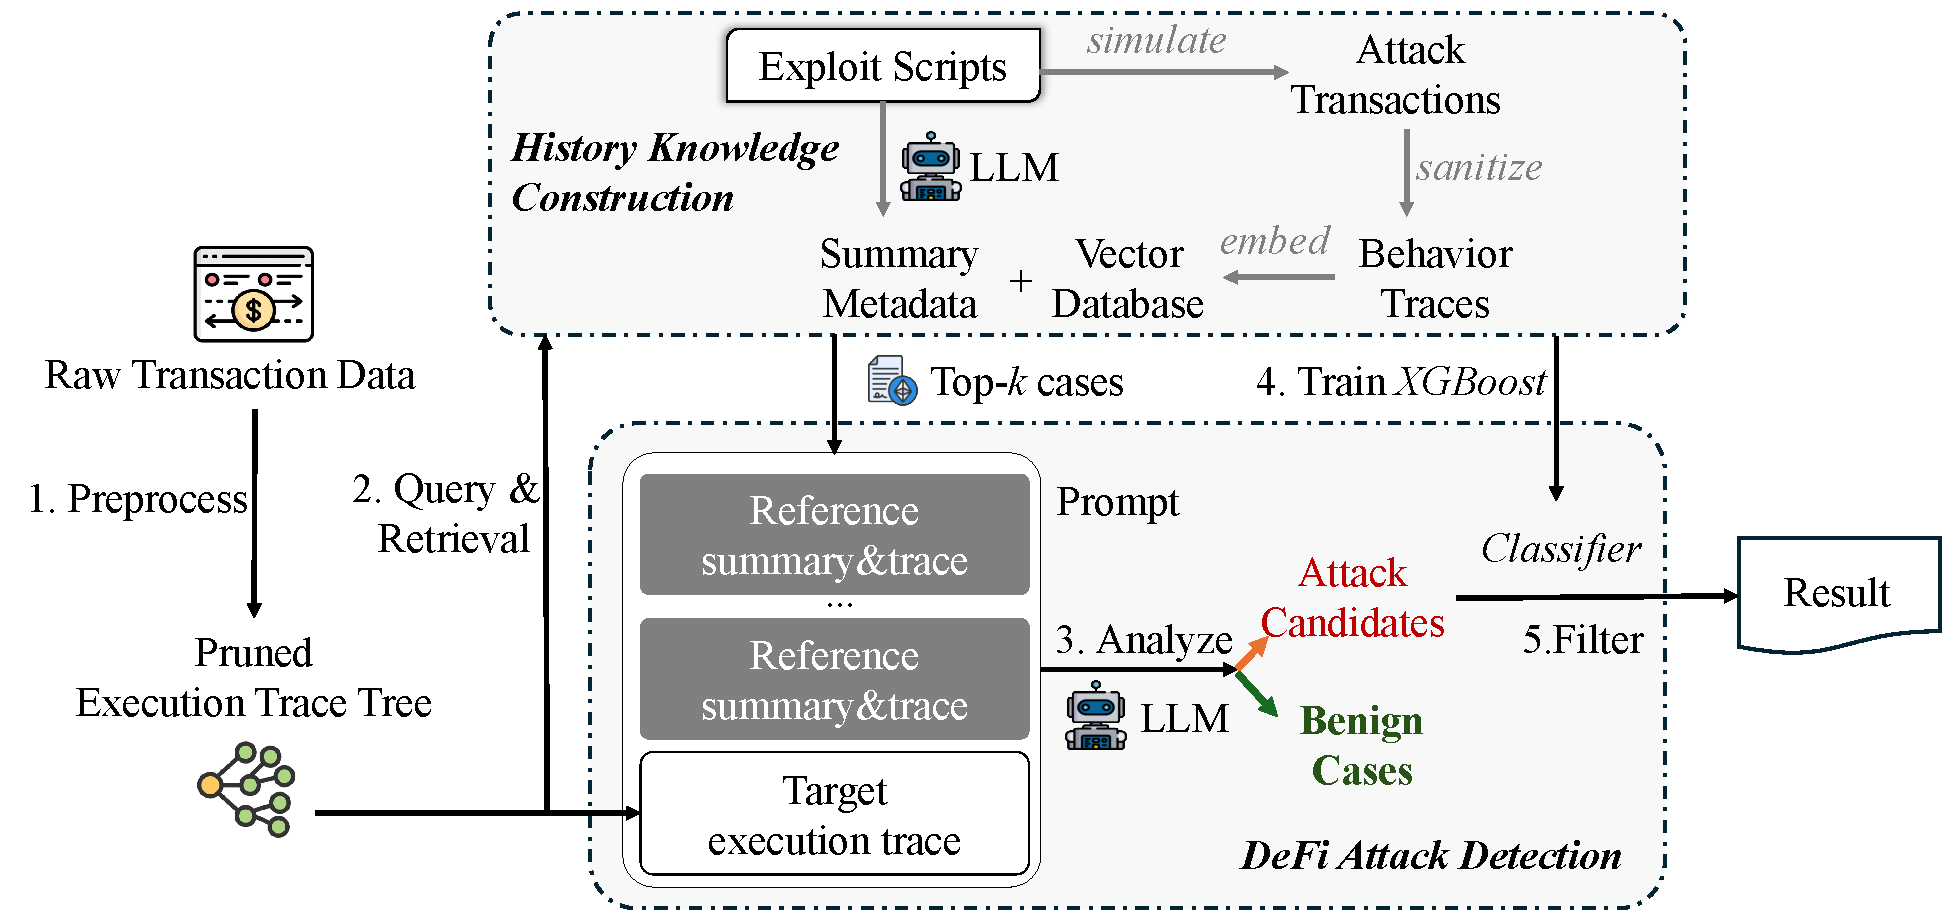
\includegraphics[width=.9\textwidth]{pic/TxHunt.pdf}
	\caption{A high-level overview of \approach}
	\label{fig:flowchart}
\end{figure*}

%\subsection{System Overview}

As illustrated in Figure~\ref{fig:flowchart}, \approach comprises two main components that work in tandem to detect DeFi attacks.

The \textit{Historical Knowledge Base} serves as an external memory that stores structured representations of past attack incidents. Unlike static rule sets, this knowledge base captures behavioral semantics---high-level descriptions of how attacks unfold---enabling \approach{} to recognize novel attack variants that share similar patterns with known incidents. The knowledge base can be incrementally expanded as new attacks are discovered and analyzed.

The \textit{RAG-based Decision Engine} processes incoming transactions through a pipeline that (1) extracts and normalizes execution traces, (2) retrieves relevant historical cases via similarity search, (3) applies a dynamic threshold to filter retrieval results, and (4) constructs prompts that guide an LLM to make attack-versus-benign decisions. The engine adapts its behavior based on retrieval results: when high-similarity historical cases exist, it leverages them for analogical reasoning; otherwise, it falls back to zero-shot analysis.

This architecture addresses the three challenges identified in Section~\ref{sec:introduction}: the knowledge base construction bridges the semantic gap (C1) by transforming low-level traces into interpretable summaries; the two-stage retrieval ensures precision (C2) by filtering out irrelevant or misleading cases; and the adaptive prompting strategy enhances reasoning reliability (C3) by grounding LLM decisions in relevant evidence.

\section{Security Knowledge Construction}
\label{sec:knowledge-base}

The knowledge base construction pipeline transforms raw historical attack data into a searchable repository of behavioral patterns. The constructions encompass three stages: execution trace minimization, semantic summarization, and vector indexing.

% \subsection{Execution Trace Collection}

We source historical attack incidents from DeFiHackLabs~\cite{defihacklabs2024}, a curated repository containing Proof-of-Concept (PoC) implementations of real-world DeFi exploits. To avoid data leakage in our experiments, we randomly sample $\sim$200 incidents to construct the knowledge base and reserve the remaining incidents for evaluation (Section~\ref{sec:evaluation}). Each PoC is a Foundry~\cite{foundry} test case that reproduces the attack on a forked blockchain state. For each incident, we execute the PoC and collect:

\begin{itemize}
    \item Invocation Flow: The sequence of external and internal function calls, including contract addresses, function signatures, and call parameters.
    \item State Changes: Modifications to contract storage, particularly balance changes for relevant tokens.
    \item Event Logs: Emitted events that signal significant operations (e.g., \texttt{Transfer}, \texttt{Swap}, \texttt{Borrow}).
    \item Metadata: Attack date, affected protocol, estimated loss, and attack type labels (when available).
\end{itemize}

The raw trace data captures the very execution details of an attack but often lacks the semantic context needed for effective analysis. 
To eliminate execution noise and reduce the trace size, we apply a minimization algorithm that removes redundant or low-information nodes while preserving the essential control-flow and asset-flow semantics of the attack.

\subsection{Execution Trace Minimization}
Raw execution traces are often complicated and verbose, resulting in overly too large context bases for LLM to reason efficiently and effectively in limited context windows.  
Our investigation reveals that exploit transactions exhibit similar execution patterns. 
First, most of them have manipulated balance of contract accounts, through the operations like \emph{send} or \emph{transfer}.
Second, many of them involve complex contract interactions through external calls, such as \emph{flashloan} that borrows a large amount of tokens from a lending protocol.
With these observations, we devise an algorithm to filter out likely unuseful items within raw execution traces while preserving attack semantics.


\begin{algorithm}[p]
\small
\caption{Execution Trace Tree Minimization}
\label{alg:trace-minimization}
\KwIn{Execution trace tree $\mathcal{T}$ with root $r$; target function
$f_t$; maximum depth $D_{\max}$; maximum argument length $L_{\max}$}
\KwOut{Minimized execution trace tree $\mathcal{T}'$}

$\mathcal{S} \gets \emptyset$\tcp*[r]{Set of previously observed call signatures}
$\textsc{MarkDuplicates}(r,\mathcal{S})$\;

$r' \gets \textsc{GeneralPrune}(r,0,D_{\max},L_{\max})$\;
\If{$r'=\varnothing$}{
    \Return $\emptyset$\;
}

$(P,d_t) \gets \textsc{FindDeepestTarget}(r',f_t)$\; \tcp*[r]{P indicates a deepest call path to the target function $f_t$ at depth $d_t$} \label{func:finddeepest}

\If{$P$ exists}{
    $\textsc{PruneTargetLevel}(r',d_t,f_t)$\; \label{func:prunetarget}
}

\Return the tree rooted at $r'$\;

% \BlankLine
\SetKwFunction{MarkDuplicates}{MarkDuplicates}
\SetKwProg{Fn}{Function}{:}{}

\Fn{\MarkDuplicates{$v,\mathcal{S}$}}{ \label{func:markduplicate:start}
    $\sigma(v) \gets \langle
        v.\mathit{type},
        v.\mathit{contract},
        v.\mathit{function},
        v.\mathit{args},
        v.\mathit{value},
        v.\mathit{return}
	\rangle$\; \label{func:markduplicate:sigma}

    \eIf{$\sigma(v)\in\mathcal{S}$}{
        $v.\mathit{duplicate}\gets\mathsf{true}$\;
    }{
        $\mathcal{S}\gets\mathcal{S}\cup\{\sigma(v)\}$\; \label{func:markduplicate:record}
    }

    \ForEach{$u\in v.\mathit{children}$}{
        $\textsc{MarkDuplicates}(u,\mathcal{S})$\;
    }  \label{func:markduplicate:end}
}

% \BlankLine
\SetKwFunction{GeneralPrune}{GeneralPrune}

\Fn{\GeneralPrune{$v,d,D_{\max},L_{\max}$}}{ \label{func:prune:start}
    \If{$v.\mathit{duplicate}=\mathsf{true}$}{ \label{func:prune:duplicate:start}
        \Return $\varnothing$\;
    } \label{func:prune:duplicate:end}

    \If{$d>D_{\max}$}{
        \Return $\textsc{TruncatedNode}(d)$\; \label{func:prune:truncated}
    }

    \If{$v.\mathit{type}=\texttt{STATICCALL}$ \textbf{and}
        $\textsc{IsMetadataQuery}(v.\mathit{function})$}{ \label{func:prune:metadata:start}
        \Return $\varnothing$\;
    } \label{func:prune:metadata:end}

    $C'\gets\emptyset$\;
    \ForEach{$u\in v.\mathit{children}$}{
        $u'\gets\textsc{GeneralPrune}(u,d+1,D_{\max},L_{\max})$\;
        \If{$u'\neq\varnothing$}{
            $C'\gets C'\mathbin{\|}u'$\;
        }
    }
    $v.\mathit{children}\gets C'$\;

    \If{$|v.\mathit{args}|>L_{\max}$}{ \label{func:prune:length}
        $v.\mathit{args}\gets
        \textsc{Prefix}(v.\mathit{args},L_{\max})
        \mathbin{\|}\texttt{<truncated>}$\;
    }

    $v.\mathit{contract}\gets\textsc{AliasAddress}(v.\mathit{contract})$\; \label{func:prune:alias}
    \Return $v$\; \label{func:prune:end}
}  

% \BlankLine
\SetKwFunction{PruneTargetLevel}{PruneTargetLevel}

\Fn{\PruneTargetLevel{$v,d_t,f_t$}}{ \label{func:prunetarget:start}
    $C'\gets\emptyset$\;
    \ForEach{$u\in v.\mathit{children}$}{
        \If{$u.\mathit{depth}\neq d_t$ \textbf{or}
            $u.\mathit{function}=f_t$}{
            $\textsc{PruneTargetLevel}(u,d_t,f_t)$\;
            $C'\gets C'\mathbin{\|}u$\;
        }
    }
    $v.\mathit{children}\gets C'$\;
} \label{func:prunetarget:end}
\end{algorithm}

% \begin{algorithm}
% 	\caption{Execution Trace Tree Minimization}\label{alg:trace}
% 	\small
% 	\begin{algorithmic}
% 		\Require $\Tau$, \emph{the tree of raw execution trace };\\
% 		\quad \quad $attackFunc$, \emph{the main function of attack script.}
% 		\Ensure $\hat{\Tau}$, \emph{the tree of minimized execution trace.}
% 		\Statex % Empty line for separation 
% 		\Procedure{Remove\_Duplicate}{$\tau$}
% 		\EndProcedure
% 		\Procedure{Prune}{$\tau$}
% 		\EndProcedure
% 		\Procedure{Extract\_Target}{$\tau$}
% 		\EndProcedure
% 		\Procedure{Main}{\Tau}
% 		\State $\hat{\Tau}$ $\gets$ $\emptyset$
% 		\For{$\tau$ in $\Tau$}
% 			\State $\hat{\tau}$ $\gets$ \textsc{Remove\_duplicate}(\tau)
% 			\State $\hat{\tau}$ $\gets$ \textsc{Prune}(\tau)
% 			\State $\hat{\Tau} =  \hat{\Tau} \cup \{\hat{\tau}\}$ 
% 		\EndFor 
% 		\For{$\tau$ in $\hat{\Tau}$}
% 		\If {not \textsc{contain\_Target}(\tau)}
% 			\State $\hat{\Tau} =  \hat{\Tau} \setminus \{\hat{\tau}\}$ 
% 		\EndIf
% 		\EndFor 
% 		\State \textbf{return} $\hat{\Tau}$
				
% 		\EndProcedure
	
% 	\end{algorithmic}
% \end{algorithm}

As shown in Algorithm~\ref{alg:trace-minimization}, the minimization process consists of three stages: duplicate removal, general pruning, and target-oriented pruning.
First, we identify repeated call nodes through a depth-first traversal (Lines~\ref{func:markduplicate:start}-\ref{func:markduplicate:end}). A call is represented by a signature tuple \emph{<type, contract, function, args, value, return>} indicating its call type, contract address, function name, arguments, transferred value, and return value (Line~\ref{func:markduplicate:sigma}). Within each trace tree, only the first occurrence of a signature is retained (Line~\ref{func:markduplicate:record}); subsequent occurrences and their subtrees are removed during pruning stage (Lines~\ref{func:prune:duplicate:start}-\ref{func:prune:duplicate:end}).

Second, we recursively apply general pruning and normalization rules (Lines~\ref{func:prune:start}-\ref{func:prune:end}). Nodes beyond the maximum traversal depth are replaced by truncation markers to preserve the existence of deeper execution while bounding the trace size~(Lines~\ref{func:prune:truncated}). We remove only low-information static metadata queries, namely calls associated with \texttt{decimals}, \texttt{symbol}, and \texttt{name}~(Lines~\ref{func:prune:metadata:start}-\ref{func:prune:metadata:end}). In contrast, other state-dependent queries such as \texttt{balanceOf} and \texttt{getReserves}, as well as event nodes, are retained because they may expose asset-flow or protocol-state evidence. 
Long argument strings are truncated to a fixed length, and contract addresses are converted to compact aliases while preserving their distinguishing prefixes and suffixes (Lines~\ref{func:prune:length}-\ref{func:prune:alias}).

Finally, we perform target-oriented structural pruning if target function(s) are given. After locating the target function \(f_t\), such as \texttt{executeOperation}, we record the depth of its first occurrence (Line~\ref{func:finddeepest}). At that depth, nodes that do not invoke \(f_t\) are removed, whereas nodes at other depths remain subject only to the general pruning rules (Line~\ref{func:prunetarget}, Lines~\ref{func:prunetarget:start}-\ref{func:prunetarget:end}). This step suppresses parallel calls that are less relevant to the monitored execution phase while retaining the context leading to the target call and its nested internal behavior. The resulting minimized tree reduces redundant and low-information content while preserving control-flow, asset-flow, and state-query evidence relevant to attack monitoring.


\subsection{Semantic Summarization and Vector Indexing}

Raw execution traces are verbose and difficult to interpret directly. We use an LLM to generate concise \textit{behavioral summaries} that describe the attack logic in natural language. The summarization prompt instructs the model to:

\begin{enumerate}
    \item Identify the attack type (e.g., price manipulation, reentrancy, access control).
    \item Describe the attack flow in 3--5 steps, focusing on the sequence of operations and their effects.
    \item Highlight key indicators: unusual fund movements, suspicious call patterns, or state manipulation.
    \item Note the vulnerability exploited and how it was triggered.
\end{enumerate}

For example, a flash-loan price manipulation attack might be summarized as: \textit{``The attacker borrows 10~M USDC via an Aave flash loan, swaps to ETH on Uniswap to inflate the ETH/USDC price, deposits ETH as collateral on the victim lending protocol (which uses Uniswap as a price oracle), borrows the maximum amount of USDC against the inflated collateral value, repays the flash loan, and profits \$2.3~M from the price discrepancy.''}
These summaries provide human-readable documentation and, more importantly, distill the semantic essence of attacks into a concise form that offers more useful context for downstream analysis and retrieval.

% \subsection{Vector Indexing}

Each attack case is stored as a record containing: (1) a unique case ID, (2) the behavioral summary, (3) the raw execution trace, and (4) structured metadata. We generate vector embeddings for the behavioral summaries using a pre-trained text embedding model and index them in a vector database.
The vector representation enables semantic similarity search: when a new transaction exhibits patterns similar to known attacks, relevant historical cases can be retrieved even if the specific contracts, function names, or token addresses differ. This ``semantic fingerprinting'' is the foundation of \approach's generalization capability.

\section{In-Context Reasoning for Attack Detection}
\label{sec:retrieval}

Na\"ive similarity search can retrieve cases that are superficially similar but semantically irrelevant, introducing noise that degrades detection accuracy. We design a two-stage retrieval mechanism to ensure high-precision context for LLM reasoning.

\subsection{Knowledge Retrieval}

Given an incoming transaction, \approach{} first preprocesses it to extract the execution trace and generates a query representation. This query is embedded using the same model as the knowledge base, and we perform approximate nearest neighbor search to retrieve the top-$k$ most similar historical cases. We compute pairwise similarity based on the L2 distance in the embedding space: $\text{sim}(q, d) = 1 - \|q - d\|_2$,
%\begin{equation}
%\text{sim}(q, d) = 1 - \|q - d\|_2
%end{equation}
where $q$ is the query embedding and $d$ is a document embedding from the knowledge base. Higher scores indicate greater semantic similarity. We set $k = 5$ to balance recall and computational efficiency.

%\subsubsection{Stage 2: Dynamic Threshold Filtering}

Not all retrieved cases are equally relevant. To filter out low-confidence matches, we apply a similarity threshold $\tau$:
$\mathcal{C}_{\text{filtered}} = \{d_i \in \text{Top-}k \mid \text{sim}(q, d_i) \geq \tau\}$.
%\begin{equation}
%\mathcal{C}_{\text{filtered}} = \{d_i \in \text{Top-}k \mid \text{sim}(q, d_i) \geq \tau\}
%\end{equation}
We empirically set $\tau = 0.85$ based on validation experiments that examined the correlation between similarity scores and detection accuracy. Cases below this threshold are discarded to prevent the LLM from being misled by tangentially related examples.

This two-stage mechanism serves as a ``quality gate'': Stage~1 casts a wide net to capture potentially relevant cases, while Stage~2 refines the results to retain only high-confidence matches. If no cases satisfy the threshold ($\mathcal{C}_{\text{filtered}} = \emptyset$), \approach{} proceeds without retrieval augmentation.

\subsection{Adaptive LLM-Based Reasoning}
\label{sec:reasoning}

The final component leverages an LLM to analyze the transaction and make an attack-versus-benign decision. We employ an adaptive prompting strategy that varies based on the retrieval results.

%\subsubsection{Retrieval-Augmented Prompt}

When closely matching historical cases are retrieved ($\mathcal{C}_{\text{filtered}} \neq \emptyset$), we construct an augmented prompt that includes:

\begin{enumerate}
    \item A \textit{role definition} establishing the LLM as an expert in smart contract attack detection.
    \item The \textit{current transaction}, i.e., the execution trace of the transaction under analysis.
    \item \textit{Historical context}: behavioral summaries and metadata of retrieved cases, with case IDs mapped to detailed security descriptions.
    \item \textit{Analysis instructions} directing the LLM to compare the current transaction against historical patterns, identify shared malicious indicators, and assess the degree of behavioral correspondence.
\end{enumerate}

\begin{figure}[t]
	\begin{tcolorbox}[title=Prompt template for retrieval-augmented detection]
		\emph{Input}:\\
		* Current transaction:  \blue{\{system\_input\}}\\
		* Historical attack examples:  \blue{\{reference\_attack\}}
		\tcbline
		You are an expert in smart contract attack detection. Your task is to analyze the Current transaction against Historical attack examples provided in the context to determine malicious intent.\\
		The historical examples were retrieved due to high behavioral similarity to the current transaction. Therefore, you must assume malicious intent initially and focus on validating the attack pattern.\\
		Following the instructions: \\
		1. Start assuming this is an Attack executing a known pattern. \\
		2. Compare execution flow and fund transfers with historical examples. \\
		3. Ignore function names; focus on operational sequence and security implications.\\
		4. Focus on Inter-contract calls, abnormal fund movements, state manipulation patterns.
		
		\tcbline
		Output MUST begin with a short answer `Attack' or `Benign', followed by below information: \\ 
		1. \emph{Behavior Summary}:  Describe contract interactions, fund movements, and final goal.
		\\
		2. \emph{Comparative Call Sequence Analysis}:  Analyze call sequence. Compare with most similar historical ID(s). State shared malicious steps.\\
		3. \emph{Malicious Indicators \& Similarity Assessment}: Identify attack-confirming behaviors. Rate similarity: High/Moderate/Low. If Benign, provide irrefutable evidence.
	\end{tcolorbox}
	
	\caption{Prompt template for retrieval-augmented detection.}
	\label{fig:prompt1}
\end{figure}


\begin{figure}[t]
	\begin{tcolorbox}[title=Prompt template for zero-shot detection]
		\emph{Input}:\\
		* Current transaction:  \blue{\{system\_input\}}
		\tcbline
		You are an expert in smart contract attack detection. Evaluate whether the current transaction is malicious based only on the provided transaction data.\\
		There is no prior knowledge or historical context provided. Following the instructions: \\
		1. Your judgment must be based purely on the internal logic, security best practices, and execution behavior of the current transaction. \\
		2. Assume the transaction is Benign unless verifiable security flaws or abnormal logic are evident in the input.\\
		\tcbline
		Output MUST begin with a short answer `Attack' or `Benign', followed by below information: \\ 
		1. \emph{Behavior Summary}:  Describe the transaction's overall behavior, including contract interactions and fund movements.
		\\
		2. \emph{Call Sequence Analysis}:  Analyze the function call sequence. Highlight unusual operations or patterns violating smart contract security practices (e.g., state change before external call).\\
		3. \emph{Malicious Indicators}: Identify behaviors indicating an attack (e.g., reentrancy, unprivileged function calls, unauthorized balance changes) OR explain why the transaction is logically sound (if Benign).
	\end{tcolorbox}
	
	\caption{Prompt template for zero-shot detection.}
	\label{fig:prompt2}
\end{figure}
%The prompt instructs the LLM to \textit{assume initial suspicion} given the proximity to known attack patterns, and to provide irrefutable evidence if concluding the transaction is benign. This design reflects the principle that close retrieval matches constitute preliminary evidence of malicious intent.
The prompt instructs the LLM to \textit{assume initial suspicion} given the proximity to known attack patterns, and to provide irrefutable evidence if concluding the transaction is benign. Concretely, a \texttt{Benign} verdict is accepted only when it is supported by explicit, trace-grounded evidence that provides concrete evidence against the malicious hypothesis suggested by retrieved cases (e.g., the absence of key malicious indicators present in the retrieved attack patterns). This design reflects the principle that close retrieval matches constitute preliminary evidence of malicious intent.

%\subsubsection{Zero-Shot Prompt}

When no cases pass the similarity threshold, \approach{} falls back to zero-shot analysis. The prompt includes only the current transaction data and general instructions for identifying suspicious patterns (e.g., reentrancy signatures, abnormal fund flows, unauthorized privilege escalation). In contrast to retrieval-augmented prompting, the zero-shot prompt adopts a conservative stance, presuming the transaction to be benign unless verifiable security flaws or anomalous execution logic are evident in the trace. This asymmetric design reflects the absence of corroborating historical evidence: without retrieval-based grounding, aggressive suspicion would increase false positives. This path handles novel attack types that lack historical analogues in the knowledge base.

%\subsubsection{Output Format}
Both prompts require the LLM to produce structured output comprising four components:
\begin{enumerate}
    \item \textit{Decision}: a binary label (\texttt{Attack} or \texttt{Benign}).
    \item \textit{Behavior Summary}: a description of the transaction's contract interactions and fund movements.
    \item \textit{Call Sequence Analysis}: an examination of function call patterns. Under retrieval augmentation, this involves comparative analysis against retrieved historical cases with an explicit assessment of behavioral correspondence; under zero-shot prompting, an independent identification of security-relevant patterns.
    \item \textit{Malicious Indicators}: specific behaviors that support the decision.
\end{enumerate}

This structured output facilitates downstream processing and provides interpretable explanations for security analysts. 

%\subsubsection{Prompt Details}
The specific prompt templates are illustrated in Figures~\ref{fig:prompt1} and Figures~\ref{fig:prompt2}: the former presents the context-aware detection prompt, which leverages retrieved historical attack instances for few-shot in-context learning; the latter details the zero-shot detection prompt, designed to evaluate transaction semantics autonomously when relevant historical references are absent.
By decoupling the reasoning logic into retrieval-augmented and zero-shot prompting, \approach{} maintains high precision for known threats while preserving the flexibility to detect novel attack types. The structured analysis fields make the LLM's reasoning process transparent, enabling security analysts to inspect the evidence chain underlying each decision.

%
%\begin{figure}[htbp]
%	\centering
%	\scalebox{0.8}{
%	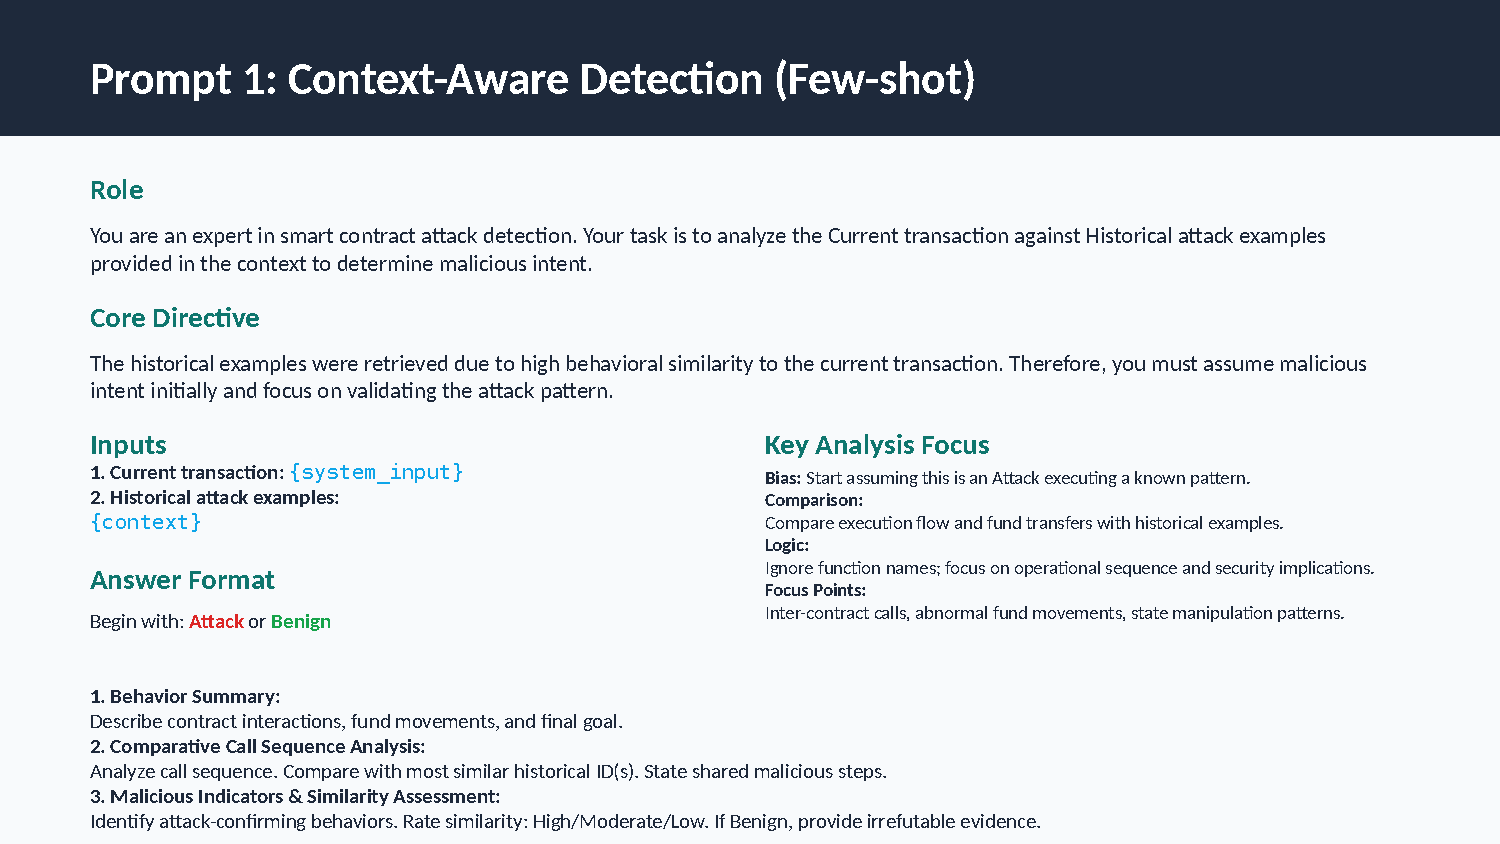
\includegraphics[width=\columnwidth,page=1]{prompts.pdf}}
%	\caption{Prompt 1: Retrieval-Augmented Detection}
%	\Description{Prompt template for retrieval-augmented detection.}
%	\label{fig:prompt1}
%\end{figure}
%
%\begin{figure}[htbp]
%	\centering
%	\scalebox{0.8}{
%	\includegraphics[width=\columnwidth,page=2]{prompts.pdf}}
%	\caption{Prompt 2: Zero-shot Detection}
%	\Description{Prompt template for zero-shot detection.}
%	\label{fig:prompt2}
%\end{figure}



\subsection{Optimization with an XGBoost Classifier}